\documentclass[aspectratio=169,t,11pt,table]{beamer}
\usepackage{../../slides}
\usepackage{../../math}
\usepackage{../../uark_colors}
\definecolor{accent}{HTML}{9D2235}
\definecolor{accent2}{HTML}{2B5269}

\title{Topic 3: Simple Linear Regression}
\subtitle{\it  ECON 4753 — University of Arkansas}
\date{Fall 2024}
\author{Prof. Kyle Butts}

\begin{document}

% ------------------------------------------------------------------------------
\begin{frame}[noframenumbering,plain]
\maketitle

% \bottomleft{\footnotesize $^*$A bit of extra info here. Add an asterich to title or author}
\end{frame}
% ------------------------------------------------------------------------------

\section{Bivariate Regression}

\begin{frame}{Covariance and Correlation}
  Recall the ways we discussed relationships between two random variables $X$ and $Y$:

  \bigskip
  Covariance, $\sigma_{XY}$ (sample analogue: $s_{XY}$)
        
  \begin{itemize}
    \item Direction matters, but magnitude is hard to interpret
  \end{itemize}
        
  \bigskip
  Correlation, $\rho_{XY}$ (sample analogue: $r_{XY}$)
  
  \begin{itemize}
    \item Direction and magnitude matter
    
    \item Correlation is always value between $[-1, 1]$
  \end{itemize}
\end{frame}

\begin{frame}{Covariance and Correlation}
  The \alert{correlation} is calculated as
  \begin{equation}\label{eq:correlation}
    r = \frac{Cov(X, Y)}{\sqrt{Var(X)} \cdot \sqrt{Var(Y)}}
  \end{equation}

  \begin{itemize}
    \item Correlation is a function of covariance, just normalizes the magnitudes so we can interpret.
  \end{itemize}
\end{frame}

\begin{frame}{Practice question}
  Suppose you calculate the sample covariance, $s_{XY} = 1.2$, and the sample standard deviations $s_X = 2$ and $s_Y = 2.5$. What is the sample correlation, $r_{XY}$?

  \begin{itemize}
    \item $0.0576$
    \item $0.24$
    \item $0.048$
    \item $4.17$
  \end{itemize}
\end{frame}


\begin{frame}{Relationship between X and Y}
  Consider this plot of NYC Math and Reading SAT Scores\only<2>{. The easiest way to summarize the relationship between $X$ and $Y$ is using a \alert{regression line}, aka the ``line of best fit''.}
  
  \medskip
  \begin{center}
    \only<1>{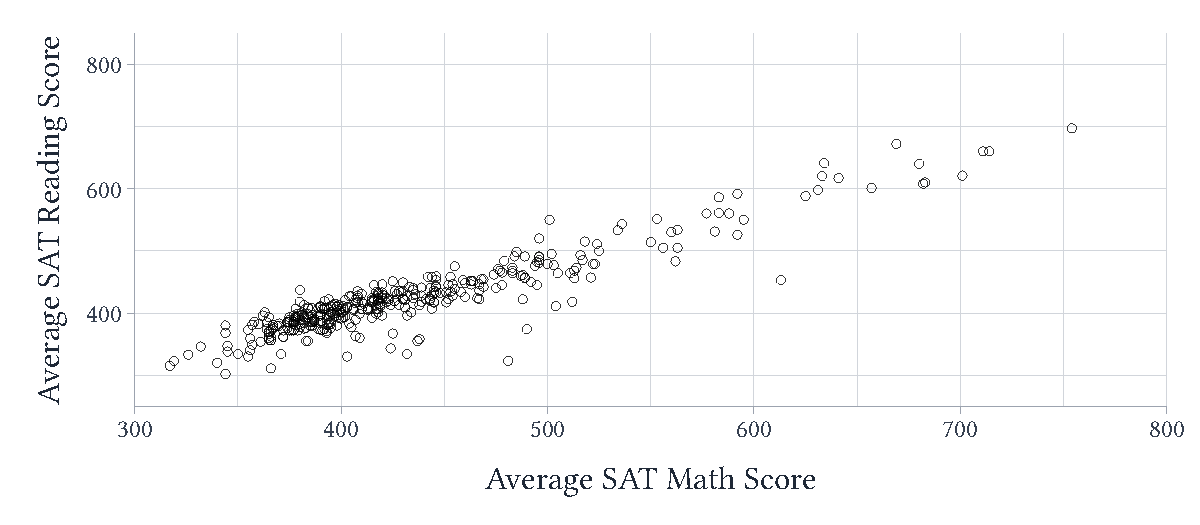
\includegraphics[width = 0.8\textwidth]{figures/nyc_sat_raw_data.pdf}}
    \only<2>{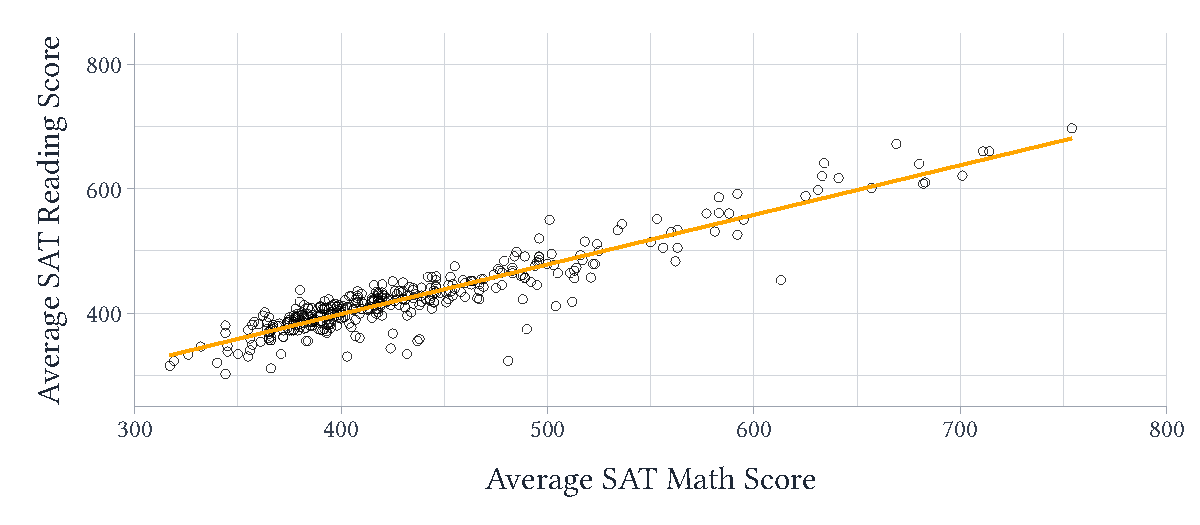
\includegraphics[width = 0.8\textwidth]{figures/nyc_sat_reg_line_of_best_fit.pdf}}
  \end{center}
\end{frame}

\begin{frame}{Regression line}
  We can write this linear model as 
  $$
    y = f(X) + \varepsilon = \beta_0 + \beta_1 * X + \varepsilon
  $$
  
  \bigskip
  The model says $y$ is a linear function of $X$. $\beta_0$ is the `intercept' and $\beta_1$ is the `slope' of the line. 
  
  \pause
  \bigskip
  We use the following terminology:
  \begin{itemize}
    \item $y$ is called `the dependent variable', `the response variable', or `the predicted variable' 
    
    \item $X$ is called `the independent variable', `the explanatory variable', `the control variable', or `the predictor variable'
  \end{itemize}
\end{frame}

\begin{frame}{Motivation for regression line}
  \vspace*{-2\bigskipamount}
  $$
    y = \beta_0 + \beta_1 * X + \varepsilon
  $$

  There are a few advantages to using a line:
  \begin{enumerate}
    \item Often time does a good job at prediction (like in our NYC example)
    \item Easy to interpret 
    \item A simple model faces less risk of overfitting the data.
  \end{enumerate}

  \bigskip
  The cost is that the model might be \emph{too simplistic} and fail to caputure many non-linear relationships between $X$ and $y$. It might yield poor predictions.
\end{frame}

\begin{frame}{Regression Line Example}
  In the previous example, the regression `line of best fit' (we will talk about how to find this line later) is given by 
  $$
    \widehat{\text{Average SAT Reading}} = 78.87 + 0.7983 * \text{Average SAT Math}
  $$
  
  The $\widehat{\quad}$ symbol means that we are \emph{predicting} average SAT reading score with our model
\end{frame}


\begin{frame}{Regression Line Example}{Predictions}
  If a school has an average SAT math score of 600, we would predict their SAT reading score would be 
  $$
    \widehat{\text{Average SAT Reading}} = 78.87 + 0.7983 * 600 = 557.85
  $$

  \pause 
  That is, our linear model would predict an average SAT reading score of 558.
\end{frame}

\begin{frame}{Slope of Line}
  How does $y$ change with $X$? Take $X$ and $X + 1$, we have the following predicted values:
  $$
    \hat{y} = \beta_0 + \beta_1 X \quad\text{ and }\quad 
    \hat{y}_{\text{new}} = \beta_0 + \beta_1 (X + 1)
  $$

  \bigskip
  So $y$ changes by 
  \begin{align*}
    \Delta y &= \left[ \beta_0 + \beta_1 (X + 1) \right] - \left[ \beta_0 + \beta_1 X \right] \\
    &= \beta_1 X + \beta_1 - \beta_1 X \\ 
    &= \beta_1
  \end{align*}

  \bigskip
  $\implies$ marginal effect of $X$ on $y$ is constant and equal to $\beta_1$
\end{frame}

\begin{frame}{Slope of Line}{Example of Constant Marginal Effects}
  \vspace*{-2\bigskipamount}
  $$
    \text{Wage} = \beta_0 + \beta_1 \text{ Education} + \varepsilon
  $$

  Implies that each year of education leads to the same change in wages
  \begin{itemize}
    \item Do you think that is reasonable?
    
    \pause
    \item Might there be a jump at high-school degree (``signaling'')?
    
    \item Returns to schooling might get smaller as we get more educated?
  \end{itemize}
\end{frame}



\begin{frame}{Prediction Error}
  Given our line, we will want to be able to evaluate how good our model does at predicting observations $y$

  \bigskip
  Define the \alert{prediction error} as 
  $$
    \hat{\varepsilon} = \underbrace{y}_{\text{true value}} - \underbrace{\hat{y}}_{\text{predicted value}} 
  $$

\end{frame}

\begin{frame}{Prediction Error}
  In the case of a linear prediction model
  $$
    \hat{\varepsilon} = \underbrace{y}_{\text{true value}} - \underbrace{\hat{y}}_{\text{predicted value}} = y - b_0 - b_1 X,
  $$
  where $b_0$ and $b_1$ are any numbers (for now).

  \bigskip
  Large $\hat{\varepsilon}$ mean you did a poor job of predicting that observation. That could be because
  \begin{enumerate}
    \item The linear model is bad at predicting $y$
    \item Or, the true noise $\varepsilon$ is making $y$ far away from the systematic component $f(X)$.
  \end{enumerate}
\end{frame}


\begin{frame}{Mean-square Error}
  Just like in Topic 2, we can form the mean-square prediction error of our linear model (in our training sample):
  $$
    \text{MSE} = \frac{1}{n} \sum_{i=1}^n (y_i - b_0 - b_1 X_i)^2
  $$

  \bigskip
  A line does a good job at predicting if MSE is (relatively) small. 

  \pause
  \bigskip
  What if we select a line based on making mean-squared prediction error as small as possible?
\end{frame}

\imageframe{figures/nyc_sat_ex_mspe_1.pdf}
\imageframe{figures/nyc_sat_ex_mspe_2.pdf}
\imageframe{figures/nyc_sat_ex_mspe_3.pdf}
\imageframe{figures/nyc_sat_ex_mspe_ols.pdf}

\begin{frame}{``Least Squares'' Regression}
  This is the basis for the \alert{ordinary least squares} regression estimator:

  $$
    \min_{\hat{\beta}_0, \hat{\beta}_1} \frac{1}{n} \sum_{i=1}^n (y_i - \hat{\beta}_0 - \hat{\beta}_1 X_i)^2
  $$

  \pause
  \bigskip
  $\hat{\beta}_0$, $\hat{\beta}_1$ are the values of the intercept and slope that minimize prediction error
  \begin{itemize}
    \item Do you see where the term ``least squares'' comes from?
  \end{itemize}
\end{frame}

\begin{frame}{Deriving Least Squares Formula}
  To minimize the function, we will take derivatives with respect to $\hat{\beta_0}$ and $\hat{\beta_1}$ and set equal to zero. First, $\hat{\beta_0}$:
  \begin{align*}
    \frac{\partial}{\partial \hat{\beta_0}} \sum_{i=1}^n (y_i - \hat{\beta_0} - \hat{\beta_1} X_i)^2 &= 0 \\
    \pause
    \implies \sum_{i=1}^n 2 (y_i - \hat{\beta_0} - \hat{\beta_1} X_i) &= 0 \\
    \implies \sum_{i=1}^n \hat{\varepsilon}_i &= 0
  \end{align*}
\end{frame}

\begin{frame}{Deriving Least Squares Formula}
  Continuing our first-order conditions for $\hat{\beta}_0$: $0 = \sum_{i=1}^n 2 (y_i - \hat{\beta_0} - \hat{\beta_1} X_i)$
  \begin{align*}
    0 &= \sum_{i=1}^n 2 (y_i - \hat{\beta_0} - \hat{\beta_1} X_i) \\
    \implies 0 &= \left(\sum_{i=1}^n y_i \right) - n \hat{\beta_0} - \left( \sum_{i=1}^n \hat{\beta_1} X_i \right) \\ 
    \pause
    \implies n \hat{\beta_0} &= \left(\sum_{i=1}^n y_i \right) - \left( \sum_{i=1}^n \hat{\beta_1} X_i \right) \\ 
    \pause
    \implies \hat{\beta_0} &= \frac{1}{n} \left(\sum_{i=1}^n y_i \right) - \hat{\beta_1} \frac{1}{n} \left( \sum_{i=1}^n X_i \right) \\ 
  \end{align*}
\end{frame}

\begin{frame}{Deriving Least Squares Formula}
  All our work lead to
  \begin{align*}
    \hat{\beta_0} = \frac{1}{n} \left(\sum_{i=1}^n y_i \right) - \hat{\beta_1} \frac{1}{n} \left( \sum_{i=1}^n X_i \right) 
  \end{align*}  

  \bigskip 
  This we can write as our first least-squares formula
  $$\hat{\beta_0} = \bar{y} - \hat{\beta_1} \bar{X}$$
\end{frame}


\begin{frame}{Deriving Least Squares Formula}
  To minimize the function, we will take derivatives with respect to $\hat{\beta_0}$ and $\hat{\beta_1}$ and set equal to zero. Second, $\hat{\beta_1}$:
  \begin{align*}
    \frac{\partial}{\partial \hat{\beta_1}} \sum_{i=1}^n (y_i - \hat{\beta_0} - \hat{\beta_1} X_i)^2 &= 0 \\
    \pause
    \implies \sum_{i=1}^n 2 X_i (y_i - \hat{\beta_0} - \hat{\beta_1} X_i) &= 0 \\
    \pause
    \implies \sum_{i=1}^n X_i \hat{\varepsilon}_i &= 0
  \end{align*}
\end{frame}

\begin{frame}{Deriving Least Squares Formula}
  Taking $\hat{\beta_0} = \bar{y} - \hat{\beta_1} \bar{X}$ and plugging into our first order condition for $\hat{\beta}_1$:
  \begin{align*}
    0 &= \sum_{i=1}^n X_i (y_i - \hat{\beta_0} - \hat{\beta_1} X_i) \\
    \implies 0 &= \sum_{i=1}^n X_i (y_i - \bar{y} + \hat{\beta_1} \bar{X} - \hat{\beta_1} X_i) \\
    \pause
    \implies 0 &= \sum_{i=1}^n X_i \left( \left( y_i - \bar{y} \right) + \hat{\beta_1} \left( \bar{X} - X_i \right) \right) \\
    \implies 0 &= \sum_{i=1}^n X_i \left( y_i - \bar{y} \right) - \hat{\beta_1} \sum_{i=1}^n X_i \left( X_i - \bar{X} \right) \\
  \end{align*}
\end{frame}

\begin{frame}{Deriving Least Squares Formula}
  \begin{align*}
    0 &= \sum_{i=1}^n X_i \left( y_i - \bar{y} \right) - \hat{\beta_1} \sum_{i=1}^n X_i \left( X_i - \bar{X} \right) \\
    \smallskip
    \implies \hat{\beta}_1 &= \frac{\sum_{i=1}^n X_i \left( y_i - \bar{y} \right)}{\sum_{i=1}^n X_i \left( X_i - \bar{X} \right)}
  \end{align*}

  With a bit of algebra, you can find:
  \begin{align*}
    \hat{\beta}_1 = \frac{\frac{1}{n} \sum_{i=1}^n \left( X_i - \bar{X} \right) \left( y_i - \bar{y} \right)}{\frac{1}{n} \sum_{i=1}^n \left( X_i - \bar{X} \right)^2} = \frac{\cov(X, y)}{\var(X)}
  \end{align*} 
\end{frame}

\begin{frame}{Least Squares Formula}
  With that, we have a formula for OLS coefficients:
  $$
    \hat{\beta}_1 = \frac{\cov(X, y)}{\var(X)} \quad\text{ and }\quad \hat{\beta}_0 = \bar{y} - \hat{\beta_1} \bar{X}
  $$

  \pause
  \bigskip
  Note that the slope $\hat{\beta}_1$ describes how $y$ changes with $X$
  \begin{itemize}
    \item That is what the covariance tells us!
  \end{itemize}
\end{frame}

\begin{frame}{Least Squares example}
  \vspace*{-\bigskipamount}
  $$
    \hat{\beta}_1 = \frac{\cov(X, y)}{\var(X)} \quad\text{ and }\quad \hat{\beta}_0 = \bar{y} - \hat{\beta_1} \bar{X}
  $$

  In our NYC example, calculate the regression coefficients of $y = $ Average SAT Reading Score and $X = $ Average SAT Math Score by hand. Here are the following statistics:
  
  
  $\cov{X, y} = 4132.97$

  $\var{X} = 5177.14$

  $\bar{X} = 432.94$

  $\bar{y} = 424.50$


  \pause
  % TODO: Answer
\end{frame}

\begin{frame}{Interpreting a Regression}

  $$
  y = \beta_0 + \beta_1 X
  $$

  \begin{itemize}
    \item $\beta_0$ is the value of $y$ whenever $X = 0$.
    
    \item $\beta_1$ is the amount $y$ changes when $X$ increases by one.
  \end{itemize}
\end{frame}

\begin{frame}{Interpreting a Regression}
  Consider this hypothetical regression:
  $$
    \hat{\text{Wins}}_i = 20.783 + 0.00913 * \text{ 3-point shots}
  $$
  
  \bigskip
  Our intercept, 20.783, is the predicted number of wings for an NBA team that shoots no 3-point shots
  
  \pause
  \bigskip
  Our slope, 0.00913, is the number of additional wins predicted for every 1 shot increase in the number of per-game 3-point shots
\end{frame}

\begin{frame}{Interpreting a Regression}
  Say we calculate the following regression line from hours studied and final exam grades:
  $$
    \widehat{\text{Final Exam}} = 38 + 5.7 * \text{Hours of Studying}
  $$

  Interpret the two regression coefficients
  \pause

  \begin{itemize}
    \item 38 is the predicted score with no studying.
    \pause
    \item Each hour of studying increases the predicted final exam score by 5.7 points.
  \end{itemize}
\end{frame}

\begin{frame}{Practice Question}
  Given that same regression line, $\widehat{\text{Final Exam}} = 38 + 5.7 * \text{Hours of Studying}$, what is the predicted final exam score if you study 8 hours?

  \pause 
  $38 + 5.7 * 8 = 83.6$
\end{frame}

\begin{frame}{Practice Question}
  A convenience store calculates a least squares line that describes how price (in dollars) of juuls affects the quantity sold; 
  $$
    \widehat{\text{Juuls sold}} = 117 - 12.4 * \text{price}
  $$ 

  If price \emph{decreases} by 1 dollar, what happens to number of juuls sold?

  \pause
  Quantity decreases by 12.4 units
\end{frame}



\begin{frame}{Algebraic properties of OLS}
  There are three properties of OLS we will cover. The first two are our first-order conditions
  \begin{enumerate}
    \item $\sum_{i=1}^n \hat{\varepsilon}_i = 0$
    \begin{itemize}
      \item The residuals sum to $0$
    \end{itemize}

    \pause
    \medskip
    \item $\sum_{i=1}^n X_i \hat{\varepsilon}_i = 0$
    \begin{itemize}
      \item The residual is uncorrelated with the $X$ variable
    \end{itemize}
    
    \pause
    \medskip
    \item $(\bar{X}, \bar{y})$ is on the regression line
  \end{enumerate}
\end{frame}

\begin{frame}{Algebraic properties of OLS}
  $(\bar{X}, \bar{y})$ is on the regression line comes from:
  \begin{align*}
    \bar{y} &= \frac{1}{n} \sum_{i=1}^n (\hat{\beta}_0 + \hat{\beta}_1 X_i + \hat{\varepsilon}_i) \\
    &= \hat{\beta}_0 + \hat{\beta}_1 \frac{1}{n} \sum_{i=1}^n X_i + \frac{1}{n} \sum_{i=1}^n \hat{\varepsilon}_i \\
    &= \hat{\beta}_0 + \hat{\beta}_1 \bar{X} + 0 \\
  \end{align*}
\end{frame}

\subsection{Prediction vs Causation}

\begin{frame}{Cautions about Correlation and Regression}
  Our regression line is fit by comparing individuals with larger and smaller $X$ values and seeing if units with larger $X$ have larger or smaller values of $y$. 

  \pause
  \bigskip
  Units with larger values of $X$ might have larger values of other variables and those other variables can affect $y$
  \begin{itemize}
    \item Which variable is driving the change in $y$? We do not know
  \end{itemize}

  Do not confuse \emph{prediction} with \emph{causation}!!! 
\end{frame}

\begin{frame}{Example of Prediction vs. Causation}
  Units with more years of schooling have higher wages
  \begin{itemize}
    \item Is this because of schooling?
    \item Or, is this because people with more schooling have higher intelligence? Differing home backgrounds? More responsible? 
  \end{itemize}

  \pause
  \bigskip\bigskip
  \begin{center}
    Correlation and regression are powerful tools for describing the relationship between two variables, but you must be careful! 
  \end{center}
\end{frame}

\begin{frame}{Correct regression interpretation}
  In general, you should use the following language:
  
  \begin{tcolorbox}[boxrule = 0pt, frame hidden, sharp corners, enhanced, borderline west = {4pt}{0pt}{green}, interior hidden]
    {\color{green}\Large $\checkmark$\ } Our regression model predicts that a one unit increase in $X$ is associated with a $\hat{\beta}_1$ units increase/decrease in $Y$
  \end{tcolorbox}

  \bigskip
  Do not say!!!!!! 
  \begin{tcolorbox}[boxrule = 0pt, frame hidden, sharp corners, enhanced, borderline west = {4pt}{0pt}{red}, interior hidden]
   {\color{red}\Large $\times$\ } Increase $X$ by one unit increases/decreases $Y$ by $\hat{\beta}_1$ units
  \end{tcolorbox}
\end{frame}

\begin{frame}{Learning about Causation}
  If you are interested in learning how to estimate \emph{causal effects}, you should take my Master's level class, ECON 5783 :-) 
\end{frame}


\section{Regression Inference}

\begin{frame}{Regression Inference}
  As we have seen, the regression coefficient $\hat{\beta}_1$ is often of interest
  \begin{itemize}
    \item Predicted change in $y$ when you increase $X$ by one unit
  \end{itemize}

  \pause
  \bigskip
  We want to be able to describe the uncertainty around this estimate. How does $\hat{\beta}_1$ change under repeated sampling?
  \begin{itemize}
    \item That is, what is the \emph{sampling distribution} of $\hat{\beta}_1$?
  \end{itemize}
\end{frame}

\imageframe{figures/ex_inference_orig_reg.pdf}
\imageframe{figures/ex_inference_extra_sample_1.pdf}
\imageframe{figures/ex_inference_extra_sample_2.pdf}
\imageframe{figures/ex_inference_extra_sample_5.pdf}
\imageframe{figures/ex_inference_extra_sample_100.pdf}
\imageframe{figures/ex_inference_sample_distribution.pdf}

\begin{frame}{Regression Inference}
  For each sample of size $n$, the regression coefficient estimate $\hat{\beta}_1$ is different
  \begin{itemize}
    \item As $n$ gets large, the noise of the estimate should get smaller
  \end{itemize}
\end{frame}

\begin{frame}{Sample Distribution of Sample Mean}
  Recall that we have the sample distribution of the sample mean (provided $n$ is `big enough'):
  $$
    \bar{X}_n \sim \mathcal{N}(\mu, \frac{\sigma^2}{n})
  $$
  \begin{itemize}
    \item What is the equivalent for regression estimates?
  \end{itemize}
\end{frame}

\begin{frame}{Sample Distribution of Regression Coefficients}
  Say the true regression line is 
  $$
      y_i = \beta_{0,0} + X_i \beta_{1,0} + \varepsilon_i
  $$
  \begin{itemize}
    \item $\beta_{0,0}$ and $\beta_{1,0}$ denotes the true regression coefficient for the population
    
    \item $\varepsilon$ is the error term from the true regression line 
  \end{itemize}

  \pause
  \bigskip
  The sampling distribution of $\hat{\beta}_1$ (for $n$ `big enough') is:
  $$
    \hat{\beta}_1 \sim 
    \mathcal{N}\left( 
      \beta_{1, 0}, \frac{ \var{\varepsilon} / n }{\var{X}} 
    \right)
  $$
\end{frame}

\begin{frame}{Sample Distribution of Regression Coefficients}
  The sampling distribution of $\hat{\beta}_1$ (for $n$ `big enough') is:
  $$
    \hat{\beta}_1 \sim 
    \mathcal{N}\left( 
      \beta_{1, 0}, \frac{ \var{\varepsilon} / n }{\var{X}} 
    \right)
  $$

  \bigskip
  Since we have a statistic $\hat{\beta}_1$ that has a sample distribution that is normally-distributed, we can do standard statistical techniques: confidence intervals, hypothesis testing, and form rejection region.  
\end{frame}

\begin{frame}{Standard Error}
  $$
    \hat{\beta}_1 \sim 
    \mathcal{N}\left( 
      \beta_{1, 0}, \frac{ \var{\varepsilon} / n }{\var{X}} 
    \right)
  $$

  \bigskip
  With this, we can calculate the \alert{standard error}, i.e. the standard deviation of the sample distribution of $\hat{\beta}_1$:
  $$
    \text{SE}(\hat{\beta}_1) = \sqrt{ \frac{ \var{\hat{\varepsilon}} / n }{\var{X}} }
  $$
  \begin{itemize}
    \item We use the residual $\hat{\varepsilon}$ because we do not observe the true error term
  \end{itemize}
\end{frame}

\begin{frame}{Standard Error}
  $$
    \text{SE}(\hat{\beta}_1) = \sqrt{ \frac{ \var{\hat{\varepsilon}} / n }{\var{X}} }
  $$

  \begin{itemize}
    \item As our sample size gets larger, $n \to \infty$, we have the distribution converges to the true value (\emph{consistency})
  \end{itemize}
\end{frame}


\begin{frame}{Confidence intervals for $\hat{\beta}_1$}
  Since we have an approximately normally distributed random variable, we can form confidence intervals just like before:

  $$
    \left[
      \hat{\beta}_1 - 1.96 * \text{SE}(\hat{\beta}_1), 
      \hat{\beta}_1 + 1.96 * \text{SE}(\hat{\beta}_1)
    \right]
  $$

  \pause
  \bigskip
  The interpretation is as before: across repeated samples, 95\% of samples' confidence intervals will contain the true value $\beta_{1, 0}$
\end{frame}

\begin{frame}{Confidence Interval Example}
  In our NYC example, the regression coefficients were $\hat{\beta}_0 = 78.87$ and $\hat{\beta}_1 = 0.798$. The standard error on $\hat{\beta}_1$ is $0.020$.

  \bigskip
  Form the 95\% confidence interval for $\hat{\beta}_1$:

  \pause
  $$
    \left[ 0.798 - 1.96 * 0.205, 0.798 + 1.96 * 0.205 \right] \approx
    \left[ 0.756, 0.837 \right]
  $$
  \begin{itemize}
    \item With 95\%, we think the true value of $\beta_1$ falls within the confidence interval $\left[ 0.756, 0.837 \right]$
  \end{itemize}
\end{frame}

\begin{frame}{Hypothesis Testing}
  Consider the test $H_0: \beta_{1, 0} = b_1$, that the slope coefficient equals $b_0$ with the (two-sided) alternative hypothesis $H_A: \beta_{1, 0} \neq b_1$

  \bigskip
  Form the \alert{test statistic}:
  $$
    \hat{t} \equiv \frac{\hat{\beta}_1 - b_1}{\text{SE}(\hat{\beta}_1)}
  $$

  With $n$ approximately large, $t$ is distributed standard-normal, and can look up the $t$-statistic in the Z-table to form the \alert{$p$-value}.
\end{frame}

\begin{frame}{Hypothesis Testing and $p$-value}
  The $p$-value tells you the probability of observing an estimate as or more extreme as the one you \emph{did} observe under the null that $\beta_{1, 0} = b_1$. So we want to look up 
  $$
    p\text{-value} = \prob{Z \leq - \abs{\hat{t}}} + \prob{Z \geq \abs{\hat{t}}} = 2 * \prob{Z \leq - \abs{\hat{t}}} 
  $$

  \pause
  \bigskip
  If $p$-value is less than the critical value (typically $0.05$), then we reject the null.
\end{frame}

\begin{frame}{Rejection Region}
  Again, we could form the 95\% confidence interval using the null value $b_1$ to find all values of $\hat{\beta}_1$ you would not reject at the 5\% significance level:

  $$
    \left[
      b_1 - 1.96 * \text{SE}(\hat{\beta}_1),
      b_1 + 1.96 * \text{SE}(\hat{\beta}_1)
    \right]
  $$
\end{frame}

% TODO: Regression in R and how to read the regression table
\begin{frame}{Regression in \texttt{R}}
  In \texttt{R}, we can do regression using the \texttt{lm} function that is built into base \texttt{R}. But we are going to use a package called \texttt{fixest} since it has a lot of extra useful features
  \begin{itemize}
    \item Install it (only need to do this once) using \texttt{install.packages("fixest")}
    
    \item At the top of your \texttt{.Rmd} files, load the pacakge using \texttt{library(fixest)}
  \end{itemize}
\end{frame}

\begin{frame}{Regression in \texttt{R}}
  You can call either \texttt{lm} or the fixest function \texttt{feols} with the exact same arguments:
  
  \texttt{feols(y \textasciitilde{} x, data = df)}
  \begin{itemize}
    \item \texttt{y \textasciitilde{} x} is the formula where \texttt{y} and \texttt{x} are the name of the variables in \texttt{df}
    \item \texttt{df} is the name you called your dataframe.
  \end{itemize}
\end{frame}

\begin{frame}[fragile]{Regression output with \texttt{feols}}
  When you run a regression, you get the following output (some lines are cut off): 

  \begin{codeblock}[{}]
                        Estimate Std. Error  t value  Pr(>|t|)
(Intercept)            78.879717   8.485841  9.29545 < 2.2e-16 ***
average_score_sat_math  0.798312   0.020525 38.89494 < 2.2e-16 ***
  \end{codeblock}

  \pause
  Each row tells you the:
  \begin{itemize}
    \item The estimate $\hat{\beta}_i$
    \item The standard error $SE(\hat{\beta}_i)$
    \item The test-statistic $\hat{t}$ for $H_0: b_i = 0$ and the corresponding p-value
  \end{itemize} 
\end{frame}

\begin{frame}[fragile]{``Stars'' in regression}
  \vspace*{-\bigskipamount}
  \begin{codeblock}[{}]
                        Estimate Std. Error  t value  Pr(>|t|)
average_score_sat_math  0.798312   0.020525 38.89494 < 2.2e-16 ***
---
Signif. codes:  0 '***' 0.001 '**' 0.01 '*' 0.05 '.' 0.1 ' ' 1
  \end{codeblock}

  \bigskip
  The stars, \texttt{*}, correspond to different levels of significance (as shown at the bottom)
  \begin{itemize}
    \item More stars means you can reject the null that $b_i = 0$ with more significance
  \end{itemize}
\end{frame}

\begin{frame}[fragile]{``Stars'' in regression}
  \vspace*{-\bigskipamount}
  \begin{codeblock}[{}]
                        Estimate Std. Error  t value  Pr(>|t|)
(Intercept)            78.879717   8.485841  9.29545 < 2.2e-16 ***
average_score_sat_math  0.798312   0.020525 38.89494 < 2.2e-16 ***
---
Signif. codes:  0 '***' 0.001 '**' 0.01 '*' 0.05 '.' 0.1 ' ' 1
  \end{codeblock}

  \bigskip
  The stars, \texttt{*}, correspond to different levels of significance (as shown at the bottom). You get stars when you reject the null at a critical value
  \begin{itemize}
    \item More stars means you can reject the null that $b_i = 0$ with more significance
  \end{itemize}

  \bigskip
  In this example, can you reject the null that the slope coefficient on the Average SAT Math Score is 0? How do you know?
\end{frame}



\section{Goodness of Fit}

\begin{frame}{$R^2$}
  We want 
  Next we define a measure to evaluate how well the regression line fits:
  $$
    R^2 = \frac{\sum_{i=1}^n (\hat{Y}_i - \bar{Y})^2}{\sum_{i=1}^n (Y_i - \bar{Y})^2} = \frac{\text{ESS}}{\text{TSS}}
  $$
  \begin{itemize}
    \item The ESS is the \alert{explained sum of squares}, i.e. the variance of the prediced $\hat{Y}$
    \item The TSS is the \alert{total sum of squares}, i.e. the variance of $Y$
  \end{itemize}
\end{frame}

\begin{frame}{Intuition of $R^2$}
  Intuitively, $R^2$ measures the percent of variation in $Y$ explained by the model
  
  $$
    R^2 = \frac{
      \text{variation in } \hat{y} \text{ along the regression line as x varies}
    }{
      \text{total variation in observed values of y}
    }
  $$
\end{frame}

\imageframe{figures/r2_comparisons.pdf}


\begin{frame}{$r$ and $R^2$}
  Correlation, $r$, describes the strength of a straight-line relationship between two variables

  \bigskip
  $R^2$, is the fraction of the variation in the values of y that is explained by the least-squares regression of $y$ on $X$. In the case of a single-variable regression, we have 
  $$
    R^2 = r^2
  $$
\end{frame}

\begin{frame}{$r$ and $R^2$}
  Lets say we have $r = -0.7786$ and $R^2 = (-0.7786)^2 = 0.6062$ between exercise and weight loss. 
  
  \begin{itemize}
    \item $r = -0.7786$, there is a strong negative linear relationship between time exercised and amount of weight gained
    
    \item $R^2 = 0.6062$, about 61\% of the variation in weight losseis accounted for by the linear relationship between weight loss and exercise. This means about 39\% of the change in weight lossed is not explained by this relationship
  \end{itemize}
\end{frame}

\begin{frame}{$R^2$ Sidebar}
  A small $R^2$ does not mean the result is uninteresting. All it means is that the $x$ variable alone does not explain a large portion of the variation in $y$.
  
  \pause
  \bigskip  
  \textbf{Example:} You find a significant relationship between exercise and income, but it has a small $R^2$. 
  
  \medskip
  We know income is determined by a variety of variables -- parent's income, education, innate ability, experience, etc. 
  
  \begin{itemize}
    \item Your result isn't uninteresting; it just means there is a lot of variation in income \emph{not due} to exercise, which is exactly what we'd expect
  \end{itemize}
\end{frame}

\begin{frame}{$R^2$ Practice Question}
  Say a researcher calculated a correlation coefficient 0.503 between SAT scores and college freshman GPA. This implies an $R^2$ of 0.253. 
  
  \bigskip
  Practice interpreting what this $R^2$ mean? 
  \begin{itemize}
    \item Does this make sense? What other things could explain the variation in freshman year GPA?
  \end{itemize}
\end{frame}

\section{Influential Observations}

\begin{frame}{Influential Observations}
  Our regression line is sensitive to \alert{outliers}, either in the $X$ or $y$ dimension 
  \begin{itemize}
    \item We say an outlier is \alert{influential} if deleting it changes our regression line substantially
    
    \item The amount by which the line changes is called the \alert{leverage} an influential observation has
  \end{itemize}
\end{frame}

\imageframe{figures/nyc_sat_reg_line_of_best_fit.pdf}
\imageframe{figures/nyc_sat_outlier.pdf}

\begin{frame}{Outliers and large samples}
  In this example, since we have a relatively large number of observations, this single outlier did not move our regression line by much
  \begin{itemize}
    \item This was one of the benefits of the regression model for $f(X)$; it does not overfit any individual observation
  \end{itemize}

  \bigskip
  Outliers tend to matter more for small samples!
\end{frame}

\begin{frame}{Outliers}
  It is always good practice to \emph{plot} the raw data. In a world full of dirty data, you will be amazed at how quickly you can spot oddities in the data

  \bigskip
  For example, \texttt{NA}s might be stored as $99$ in a dataset
  \begin{itemize}
    \item While one single outlier might not move the regression line by much, a large number of them will!!
  \end{itemize}
\end{frame}


\section{Discrete Variables}

\begin{frame}{Discrete Variables}
  So far, we have thought about $X$ variables that are continuously distributed. Now, we turn to the other extreme where $X$ is a discrete variable
  \begin{itemize}
    \item Remember, \alert{discrete} means the variable takes on finitely many values
  \end{itemize}
\end{frame}

\begin{frame}{Regression and Sample Means}
    First, we will have an aside on a sort-of peculiar regression: 
    \texttt{lm(y \textasciitilde{} 1, data = df)}
    \begin{itemize}
      \item Regress \texttt{y} on a variable that is equal to 1 for all observations
    \end{itemize}

    \pause
    \bigskip
    This model is written as $y_i = \alpha + u_i$. What is the best estimate of $\hat{\alpha}$?
    \begin{itemize}
      \item Well, we observe \emph{no} information about the individual, so our best guess at $y_i$ is the sample mean of $y$ $\implies \hat{\alpha} = \bar{y}$
    \end{itemize} 
\end{frame}

\begin{frame}[fragile]{}
  \begin{codeblock}
library(fixest)
feols(mpg ~ 1, data = mtcars)
#> OLS estimation, Dep. Var.: mpg
#> Observations: 32
#> Standard-errors: IID 
#>             Estimate Std. Error t value  Pr(>|t|)    
#> (Intercept)  20.0906    1.06542 18.8569 < 2.2e-16 ***
#> ---
#> Signif. codes:  0 '***' 0.001 '**' 0.01 '*' 0.05 '.' 0.1 ' ' 1
#> RMSE: 5.93203

mean(mtcars[["mpg"]])
#> [1] 20.09062
  \end{codeblock}
\end{frame}

\begin{frame}{Regression and Sample Means}
  \begin{center}
    \texttt{feols(y \textasciitilde{} 1, data = df)}
  \end{center}

  \bigskip
  Running this regression is useful because it will estimate the mean of \texttt{y} and give us the standard error estimate $\frac{\sigma}{\sqrt{n}}$
  \begin{itemize}
    \item This makes inference easier: hypothesis testing and confidence intervals 
  \end{itemize}
\end{frame}

\begin{frame}{Indicator variable}
  We now understand the simplest regression on just an intercept. What about an \alert{indicator variable}? 
  
  An \emph{indicator variable} is a variable that can only equal $0$ and $1$
  \begin{itemize}
    \item $X$ "indicates" when a unit is of type 0 or type 1
  \end{itemize}

  \bigskip
  E.g. include being born male (=1) or female (=0); being White (=1) or not (=0); having a high-school degree (=1); being over 6 foot tall (=1) or under (=0); etc.
\end{frame}

\begin{frame}{Indicator variable}
  Let's work through some properties of an indicator variable. First, The sample mean of an indicator variable is the proportion of units with a 1:
  $$
    \frac{1}{n} \sum_{i=1}^n X_i \pause = \frac{\# \text{ of } 1{s}}{n} = \text{\% of sample with 1}
  $$
  
  Define $\pi$ as the fraction of units with $X_i = 1$ 

  \pause
  \bigskip
  Second, I'll assert without proof (write down the formula and you can figure it out):
  $$
    \var(X_i) = \pi (1 - \pi)
  $$
\end{frame}

\begin{frame}{Covariance with an indicator variable}
  What is $\cov(X_i, Y_i)$? Rembmer
  $$
    \cov(X_i, Y_i) = \expec{X_i Y_i} - \expec{X_i} \expec{Y_i}
  $$
  
  \pause
  \bigskip
  Again, skipping the math:
  \begin{align*}
    \cov(X_i, Y_i) = \pi (1 - \pi) \left( \expec{Y_i}{X_i = 1} - \expec{Y_i}{X_i = 0} \right)
  \end{align*}
\end{frame}

\begin{frame}{Covariance with an indicator variable}
  Math details (if you're curious): 
  \begin{align*}
    \cov(X_i, Y_i) 
    &= \expec{X_i Y_i} - \expec{X_i} \expec{Y_i} \\
    &= \expec{X_i Y_i} - \pi \left( \pi \expec{Y_i}{X_i = 1} + (1 - \pi) \expec{Y_i}{X_i = 0} \right) \\
    &= \pi \expec{Y_i}{X_i = 1} - \pi \pi \expec{Y_i}{X_i = 1} - \pi (1 - \pi) \expec{Y_i}{X_i = 0} \\
    &= \pi (1 - \pi) \left[ \expec{Y_i}{X_i = 1} - \expec{Y_i}{X_i = 0} \right]
  \end{align*}
\end{frame}

\begin{frame}{Regression with an indicator variable}
  Say you have a regression of $Y_i = \beta_0 + \beta_1 * X_i + u_i$. What does $\hat{\beta}_0$ and $\hat{\beta}_1$ equal?

  \begin{align*}
    \hat{\beta}_1 
    &= \frac{\cov(X_i, Y_i)}{\var{X_i}} \\ \pause
    &= \frac{\pi (1 - \pi) \left( \expec{Y_i}{X_i = 1} - \expec{Y_i}{X_i = 0} \right)}{\pi (1 - \pi)} \\
    &= \expec{Y_i}{X_i = 1} - \expec{Y_i}{X_i = 0}
  \end{align*}
  
  The coefficient $\hat{\beta}_1$ tells me the difference in sample means between the group with $X_i = 1$ and the group with $X_i = 0$
\end{frame}

\begin{frame}{Regression with an indicator variable}
  Say you have a regression of $Y_i = \beta_0 + \beta_1 * X_i + u_i$. From the last slide, we have:
  $$ 
    \hat{\beta}_1 = \expec{Y_i}{X_i = 1} - \expec{Y_i}{X_i = 0} 
  $$

  \bigskip
  Solving our other first-order condition for $\hat{\beta}_0$, we have:
  \begin{align*}
    \hat{\beta}_0 = \expec{Y_i}{X_i = 0}
  \end{align*}
\end{frame}

\begin{frame}{Math Details}
  \begin{align*}
    \beta_0 &= \expec{Y} - \hat{\beta}_1 \expec{X} \\
    &= \expec{Y} - \hat{\beta}_1 \pi \\
    &= \pi \expec{Y_i}{X_i = 1} + (1 - \pi) \expec{Y_i}{X_i = 0} - \pi \expec{Y_i}{X_i = 1} - \pi \expec{Y_i}{X_i = 0} \\
    &= \expec{Y_i}{X_i = 0}
  \end{align*}
\end{frame}

\begin{frame}{Interpreting the coefficients}
  Our model (without the error term) is $\hat{Y}_i = \beta_0 + \beta_1 X_i$.

  \bigskip
  Since $X_i$ contains only two values, we can just compare them directly:
  \begin{itemize}
    \item When $X_i = 0$, $\hat{Y}_i = \beta_0 + \beta_1 * 0 = \beta_0$
    
    \pause
    \item When $X_i = 1$, $\hat{Y}_i = \beta_0 + \beta_1 * 1 = \beta_0 + \beta_1$
  \end{itemize}

  \bigskip
  $\beta_0$ is our predicted value for $Y_i$ for the group with $X_i = 0$ and $\beta_0 + \beta_1$ is our predicted value for $Y_i$ for the group with $X_i = 1$ 
\end{frame}

\begin{frame}{Intuition}
  $\beta_0$ is our predicted value for $Y_i$ for the group with $X_i = 0$ and $\beta_0 + \beta_1$ is our predicted value for $Y_i$ for the group with $X_i = 1$ 

  \bigskip
  Given this, then our regression coefficients make sense:
  \begin{itemize}
    \item $\hat{\beta}_0$ is the average value of $Y_i$ for the group with $X_i = 0$
    
    \item $\hat{\beta}_1$ is the difference in the means between the two groups
    
    \item This makes $\hat{\beta}_0 + \hat{\beta}_1$ is the average value of $Y_i$ for the group with $X_i = 1$
  \end{itemize}
\end{frame}

\begin{frame}{Example}
  Let's revisit our example with the \texttt{mtcars} dataset. There is an indicator variable, \texttt{am} for being an automatic (=1) or manual (=0). 
  Regress the miles per gallon a car gets, \texttt{mpg}, on \texttt{am}.

  \begin{itemize}
    \item In \texttt{fixest}, we can use \texttt{i(am)} to make it print out more nicely
  \end{itemize}
\end{frame}
 
\begin{frame}[fragile]{}
  \begin{codeblock}
feols(mpg ~ i(am), data = mtcars)
#> OLS estimation, Dep. Var.: mpg
#> Observations: 32
#> Standard-errors: IID 
#>             Estimate Std. Error  t value   Pr(>|t|)    
#> (Intercept) 17.14737    1.12460 15.24749 1.1340e-15 ***
#> am::1        7.24494    1.76442  4.10613 2.8502e-04 ***

mean(mtcars[mtcars$am == 1, ]$mpg)
#> [1] 24.39231
mean(mtcars[mtcars$am == 0, ]$mpg)
#> [1] 17.14737
  \end{codeblock}
\end{frame}


\begin{frame}{Multi-valued discrete variables}
  This intuition will extend directly to settings where we have a discrete variable that obtains $K$ distinct values:
  \begin{itemize}
    \item E.g. race, 10-year bins of age, number of cylinders in engine
  \end{itemize}

  \pause
  \bigskip
  We can construct a \emph{set of} indicator variables for each value that $X$ can obtain. For $k = 1, \dots, K$
  $$
    X_{ik} \equiv \one{X_i = x_k}
  $$
  \begin{itemize}
    \item $K$ such variables $X_{i1}, \dots, X_{iK}$
  \end{itemize}
\end{frame}

\begin{frame}{Multi-valued variable regression}
  Now we are in a setting where we have multiple regressors on the right-hand side ($K$ indicators). 
  $$
    y_i = \sum_{k=1}^K X_{ik} \beta_k + u_i
  $$

  \pause
  \bigskip
  We don't know what these regressions estimate yet
  \begin{itemize}
    \item Note we are in a very special case since these variables are mutually exclusive (only one of them is non-zero per unit)
  \end{itemize}
\end{frame}

\begin{frame}{Multi-valued variable regression}
  \vspace*{-\bigskipamount}
  $$
    y_i = \sum_{k=1}^K X_{ik} \beta_k + u_i
  $$

  From the same intuition as before, we have $\hat{\beta}_k$ is the sample average of $y_i$ for individuals with $X_i = x_k$
\end{frame}

\begin{frame}{Example}
  Let's revisit our example with the \texttt{mtcars} dataset. Let's see if \texttt{mpg} differs based on the number of cylinders a car has, \texttt{cyl}. 

  \begin{itemize}
    \item In \texttt{fixest}, we can use \texttt{i(am)} to make indicators for each value of a variable

    \item Otherwise, we could for $4$, $6$, and $8$ create the indicator variables with \texttt{mtcars\$cyl4 = (mtcars\$cyl == 4)}
  \end{itemize}
\end{frame}

\begin{frame}[fragile]{}
  Interpret these coefficients:

  \begin{codeblock}
library(fixest)
feols(mpg ~ 0 + i(cyl), data = mtcars)
#> OLS estimation, Dep. Var.: mpg
#> Observations: 32
#> Standard-errors: IID 
#>        Estimate Std. Error t value   Pr(>|t|)    
#> cyl::4  26.6636   0.971801 27.4373  < 2.2e-16 ***
#> cyl::6  19.7429   1.218217 16.2064 4.4933e-16 ***
#> cyl::8  15.1000   0.861409 17.5294  < 2.2e-16 ***
#> ---
#> Signif. codes:  0 '***' 0.001 '**' 0.01 '*' 0.05 '.' 0.1 ' ' 1
#> RMSE: 3.0683   Adj. R2: 0.704784
  \end{codeblock}
\end{frame}

\begin{frame}{Intercept and Multicollinearity}
  In the future, we will want to include many right-hand side variables (beyond our multi-valued discrete variable). In this case, we want to include an \emph{intercept}

  \bigskip
  $$
    y_i = \alpha + \sum_{k=1}^K X_{ik} \beta_k + u_i
  $$
\end{frame}

\begin{frame}[fragile]{Multicollinearity}
  Our $X$ variables look like this. Note the 3 \texttt{cyl} indicator variables sum to the intercept
  \begin{codeblock}
#> (Intercept)   cyl::4   cyl::6   cyl::8
#>           1        0        1        0
#>           1        0        1        0
#>           1        1        0        0
#>           1        0        1        0
#>           1        0        0        1
#>           1        0        1        0
#>           1        0        0        1
#>           1        1        0        0
  \end{codeblock}
\end{frame}

\begin{frame}{Multicollinearity}
  \vspace*{-\bigskipamount}
  $$
    \hat{y}_i = \hat{\alpha} + \sum_{k=1}^K X_{ik} \hat{\beta}_k 
  $$
  It turns out that we face a non-uniqueness problem because of the \alert{multicollinearity} we identified 
  \begin{itemize}
    \item We can add 10 to $\hat{\alpha}$ and subtract 10 from $\hat{\beta}_4$, $\hat{\beta}_6$, and $\hat{\beta}_8$ and get the same $\hat{y}$
  \end{itemize}

  \bigskip
  Therefore, we will typically need to drop one of the $X_{ik}$ variables (or \texttt{R} will do it for you)
\end{frame}

\begin{frame}[fragile]{}
  \begin{codeblock}
library(fixest)
feols(mpg ~ 1 + i(cyl), data = mtcars)
#> OLS estimation, Dep. Var.: mpg
#> Observations: 32
#> Standard-errors: IID 
#>              Estimate Std. Error  t value   Pr(>|t|)    
#> (Intercept)  26.66364   0.971801 27.43735  < 2.2e-16 ***
#> cyl::6       -6.92078   1.558348 -4.44110 1.1947e-04 ***
#> cyl::8      -11.56364   1.298623 -8.90453 8.5682e-10 ***
#> ---
#> Signif. codes:  0 '***' 0.001 '**' 0.01 '*' 0.05 '.' 0.1 ' ' 1
#> RMSE: 3.0683   Adj. R2: 0.714009
  \end{codeblock}
\end{frame}

\begin{frame}{Interpreting Multicollinearity}
  In the previous example, we dropped $\one{X_i = 4}$. This is the \alert{omitted group}. What happened to our coefficient estimates?

  \bigskip
  \begin{itemize}
    \item Just like in the indicator variable case, $\hat{\alpha}$ estimated the mean of \texttt{mpg} for cars with $X_i = 4$
    
    \pause
    \item The coefficients on the other $\hat{\beta}_k$ now represent the \emph{difference} in means between the group for $X_i = 6$ and the `omitted group' $X_i = 4$. 
    \begin{itemize}
      \item The mean for $X_i = 6$ is $19.742 = 26.663 - 6.921$
    \end{itemize}
  \end{itemize}
\end{frame}

\begin{frame}[fragile]{Specifying \texttt{ref} option}
  \vspace*{-1.25\bigskipamount}
  \begin{codeblock}
library(fixest)
feols(mpg ~ i(cyl, ref = 6), data = mtcars)
#> OLS estimation, Dep. Var.: mpg
#> Observations: 32
#> Standard-errors: IID 
#>             Estimate Std. Error  t value   Pr(>|t|)    
#> (Intercept) 19.74286    1.21822 16.20636 4.4933e-16 ***
#> cyl::4       6.92078    1.55835  4.44110 1.1947e-04 ***
#> cyl::8      -4.64286    1.49200 -3.11182 4.1522e-03 ** 
#> ---
#> Signif. codes:  0 '***' 0.001 '**' 0.01 '*' 0.05 '.' 0.1 ' ' 1
#> RMSE: 3.0683   Adj. R2: 0.714009
  \end{codeblock}
\end{frame}

\begin{frame}[fragile]{Significance with indicator variables}
  \vspace*{-1.25\bigskipamount}
  \begin{codeblock}
#>              Estimate Std. Error  t value   Pr(>|t|)    
#> (Intercept)  26.66364   0.971801 27.43735  < 2.2e-16 ***
#> cyl::6       -6.92078   1.558348 -4.44110 1.1947e-04 ***
#> cyl::8      -11.56364   1.298623 -8.90453 8.5682e-10 ***
#> ---
#> Signif. codes:  0 '***' 0.001 '**' 0.01 '*' 0.05 '.' 0.1 ' ' 1
  \end{codeblock}
  
  Including an intercept also helps with certaint statistical inference.
  The estimates test that the average of $y$ for the omitted group is \emph{the same} for the other groups
  \begin{itemize}
    \item Rejecting this ($p$-value $< \alpha$) rejects the null that the two means are the same
  \end{itemize}
\end{frame}


\section{\texorpdfstring{$\log$}{log} transformations}

\begin{frame}{$\log$-transformation}
  In economics, it is common to see $\log$ transformed outcomes: 
  $$
    \log(w_i) = \beta_0 + \beta_1 \text{College Degree}_i + u_i
  $$
  \pause
  This specification changes our interpretation of the slope coefficients:

  \bigskip
  Having a college degree is associated with an increase in wages of $\beta_1 * 100$ percent
  \begin{itemize}
    \item E.g. if $\beta_1 = 0.02$, then a college degree is associated with a 2\% increase in wages.
  \end{itemize}
\end{frame}

\begin{frame}{Derivation of $\log$-transformation interpretation}
  Compare two individuals: unit $1$ with and unit $0$ without a college degree. Then, we have 
  \begin{align*}
    \log(w_1) - \log(w_0) &= \beta_0 + \beta_1 - \beta_0 \\
    \implies \log(w_1 / w_0) &= \beta_1 \\
    \implies \log(1 + \frac{w_1 - w_0}{w_0}) &= \beta_1
  \end{align*}

  \pause
  \bigskip
  If you recall, exponentiating gets rid of the the $\log$
  $$
    \frac{w_1 - w_0}{w_0} = \exp(\beta_1) - 1
  $$
\end{frame}

\begin{frame}{Derivation of $\log$-transformation interpretation}
  \vspace*{-\bigskipamount}
  $$
    \frac{w_1 - w_0}{w_0} = \exp(\beta_1) - 1
  $$
  The left-hand side is our percent-change formula from high-school science class

  \pause
  \bigskip
  In this case, the more \emph{precise} answer is that having a college degree is associated with an $\exp(\beta_1) - 1$ percent change in $w$
  \begin{itemize}
    \item But for $-0.10 < \beta_1 < 0.10$, $\exp(\beta_1) - 1$ is approximately equal to $\beta_1$ so it's simpler to use the latter
  \end{itemize}
\end{frame}

\imageframe{figures/pct_change_approximation.pdf}


\begin{frame}{Example}

\end{frame}

\imageframe{figures/ex_log_y_raw.pdf}
\imageframe{figures/ex_log_y_log_vs_linear.pdf}

% \begin{frame}{Example in \texttt{R}}
%   \begin{codeblock}
% library(fixest)
% feols(log(hp) ~ i(cyl), data = mtcars)
% #> OLS estimation, Dep. Var.: log(hp)
% #> Observations: 32
% #> Standard-errors: IID 
% #>             Estimate Std. Error  t value   Pr(>|t|)    
% #> (Intercept) 4.383896   0.069759 62.84353  < 2.2e-16 ***
% #> cyl::6      0.408183   0.111863  3.64895 1.0282e-03 ** 
% #> cyl::8      0.934249   0.093219 10.02206 6.2778e-11 ***
% #> ---
% #> Signif. codes:  0 '***' 0.001 '**' 0.01 '*' 0.05 '.' 0.1 ' ' 1
% #> RMSE: 0.220252   Adj. R2: 0.762984
%   \end{codeblock}
% \end{frame}

\begin{frame}{When to use $\log$ transformations}
  You should take the $\log$ of an outcome varible when you think a 1 unit change in $X$ is related to a \% change in $Y$. 

  \pause
  \bigskip
  $\log(Y)$ \textasciitilde{} $X$ is called fitting an `exponential' relationship. These are common in:
  \begin{enumerate}
    \item Financial markets where compounding returns imply $Y_t = Y_0 e^{rt}$
    
    \item Epidemiology where disease growth rate is exponential (it is not actually, but early growth rate is approximately)
    
    \pause
    \item Settings with skewed distributions (e.g. home prices, GDP, population)
    \begin{itemize}
      \item Skewness makes a `unit' change in $X$ difficult to think about
    \end{itemize}
  \end{enumerate}
\end{frame}

\begin{frame}{$\log$-$\log$ transformations}
  Alternatively, You may see $\log$ transformations of both variables:
  $$
    \log(Y_i) = \beta_0 + \beta_1 \log(X_i) + u_i
  $$

  \bigskip
  The interpretation is now simpler: a 1\% change in $X_1$ is associated with a $\beta_1$ \% change in $Y$
\end{frame}

% \begin{frame}{Example in \texttt{R}}
%   \begin{codeblock}
% library(fixest)
% feols(log(mpg) ~ log(hp), data = mtcars)
% #> OLS estimation, Dep. Var.: log(mpg)
% #> Observations: 32
% #> Standard-errors: IID 
% #>              Estimate Std. Error  t value   Pr(>|t|)    
% #> (Intercept)  5.545381   0.299133 18.53821  < 2.2e-16 ***
% #> log(hp)     -0.530092   0.060994 -8.69086 1.0796e-09 ***
% #> ---
% #> Signif. codes:  0 '***' 0.001 '**' 0.01 '*' 0.05 '.' 0.1 ' ' 1
% #> RMSE: 0.156265   Adj. R2: 0.706247
%   \end{codeblock}
% \end{frame}





\end{document}
